\section{Cipher Specifications}

\begin{frame}{Cipher Specifications}
\begin{block}{}
    \begin{itemize}
        \item Lightweight Block Cipher
        \item Bit-Slice Style
        \item Competetive Software Performance
        \item Hardware Friendly
        \item Very Strong Security
    \end{itemize}
\end{block}
\end{frame}

\begin{frame}{THE ROUND TRANSFORMATION}
\begin{block}{}
    \begin{itemize}
        \item AddRoundkey(ARK)
        \item SubColumn(SC)
        \item ShiftROw(SR)
        \item KeySchedule(KS)
    \end{itemize}
\end{block}
\end{frame}


\begin{frame}
\begin{block}{Pseudo-Code-}
    \textbf{GenerateRoundKeys(state)}:\\
\hspace*{1cm}\textbf{for i = 0 to 24 do:}\\
\hspace*{2cm}\textbf{ARK(state,$K_i$)}\\
\hspace*{2cm}\textbf{SC(state)}\\
\hspace*{2cm}\textbf{SR(state)}\\
\hspace*{1cm}\textbf{ARK(state,$K_{25}$)}\\
    \end{block}
\end{frame}



\begin{frame}
\begin{block}{Shorter Visualization}
    \centering
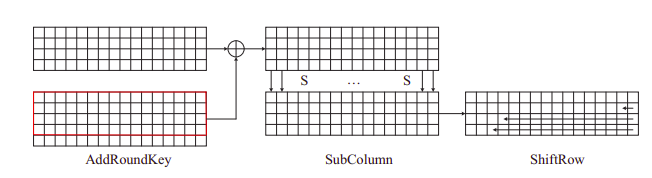
\includegraphics[width=8cm]{img_13.png}
\centering
    \end{block}
\end{frame}

\begin{frame}{Differential Distribution Table (DDT)
}
\begin{block}{}
\centering
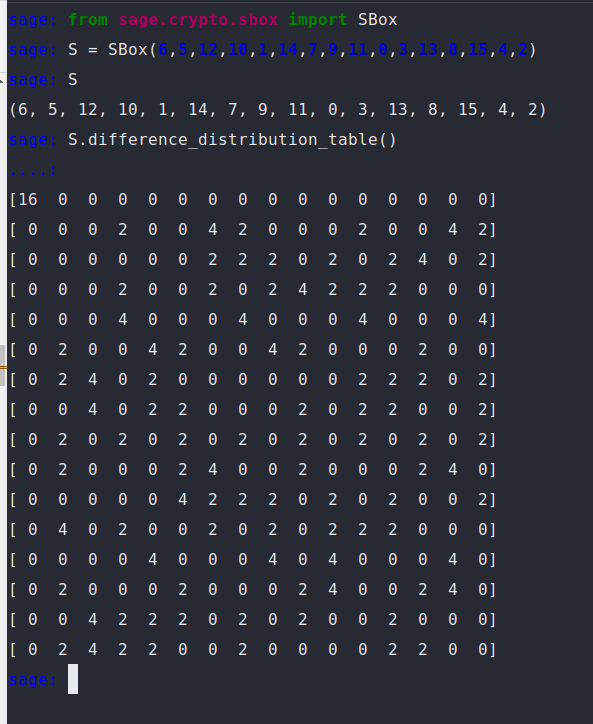
\includegraphics[width=50mm]{img_1.png}
\centering
\end{block}
    
\end{frame}


\begin{frame}{Linear Approximation Table (LAT)
}
\begin{block}{}
\centering
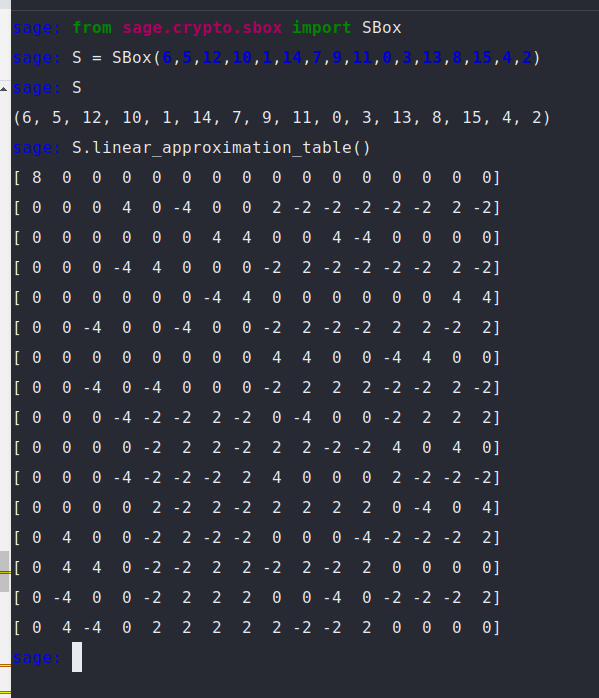
\includegraphics[width=50mm]{img_2.png}
\centering
\end{block}
    
\end{frame}

\begin{frame}{Key Schedule}
    \begin{block}{For 80-bit key}
    \begin{enumerate}
        \item SC to the bits at the 4 uppermost rows and the 4 rightmost
columns
\item Using a 1-round generalized Feistel transformation\\
Row’0 := (Row0 << 8) $\oplus$ Row1\\
Row’1 := Row2\\
Row’2 :=Row3\\
Row’3 := (Row3 << 12) $\oplus$ Row4\\
Row’4 := Row0
\item A 5-bit round constant RC[i] is XORed with the 5-bit key
state for i $\in$ (1,2,..,24).
    \end{enumerate}
        
    \end{block}
    
\end{frame}
\begin{frame}{Key Schedule}
    \begin{block}{For 80-bit key}
    \begin{enumerate}
    \item SC to the bits at the 8 rightmost columns.
    \item Using a 1-round generalized Feistel transformation\\
    Row’0 := (Row0 << 8) $\oplus$ Row1\\
    Row’1 := Row2\\
    Row’2 := (Row2 << 16) $\oplus$ Row3 
    Row’3 := Row0
    \item A 5-bit round constant is XORed with the 5-bit key state
    \end{enumerate}
    \end{block}
\end{frame}

\begin{frame}{Security Analysis}
\begin{block}{Integral Cryptanalysis}
\begin{itemize}
    \item We implemented the Square attack which used a 4-round integral distinguisher
    \item Encryption : After 4-rounds, the XOR sum in any 4 bit positions equals to 0, i.e. (Balanced property)
$\oplus$ S4[0] = $\oplus$ S4[17] = $\oplus$ S4[43] = $\oplus$ S4[60] = 0
    \begin{block}{}
\centering
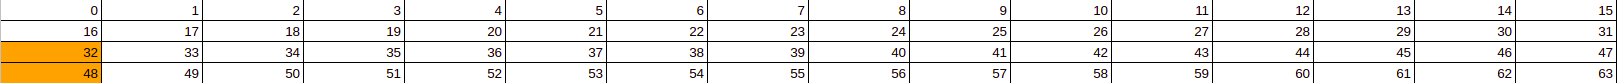
\includegraphics[height=1cm,width=100mm]{img_5.png}
\centering
\end{block}
\item Decryption : We choose $2^{48}$ plaintexts s.t. cols - 0, 13, 14, 15 maintain CONSTANT property and other 12 cols maintain the ALL property.
\item $2^{48}$ Intermediate values ⇒ $2^{47}$ subsets ⇒ 2 values.
\item 4 → 7 → 25 rounds with same integral distinguisher.
\end{itemize}
\end{block}
\end{frame}

\begin{frame}{SECURITY ANALYSIS}
\begin{block}{Differential Cryptanalysis}
\begin{itemize}
    \item Differential Cryptanalys is strongest techniques for the
cryptanalysis of block ciphers
    \item Using the algorithm based on the branch and bound method,
the best differential trails from round-1 to round-15 were
found.
    \begin{block}{}
    \tiny
    \centering
\begin{array}{||c|c||c|c||c|c||}
\hline \sharp R & \text { Prob. } & \sharp \mathrm{R} & \text { Prob. } & \sharp \mathrm{R} & \text { Prob. } \\
\hline 1 & 2^{-2} & 6 & 2^{-18} & 11 & 2^{-46} \\
\hline 2 & 2^{-4} & 7 & 2^{-25} & 12 & 2^{-51} \\
\hline 3 & 2^{-7} & 8 & 2^{-31} & 13 & 2^{-56} \\
\hline 4 & 2^{-10} & 9 & 2^{-36} & 14 & 2^{-61} \\
\hline 5 & 2^{-14} & 10 & 2^{-41} & 15 & 2^{-66} \\
\hline
\end{array}
\centering
\end{block}
    \item Using the 14-round differential propagation, we can mount an
attack on 18-round Rectangle cipher
    \item 25-round Rectangle is enough to behold out against this
differential cryptanalysis attack.
    
\end{itemize}
    
\end{block}
    
\end{frame}